\subsection{BÀI TẬP TRẮC NGHIỆM}
\Opensolutionfile{ans}[ans/ansTL-CD2]
\setcounter{ex}{0}
\boxmini{ĐỀ SỐ 1}
\begin{ex}
	Kí hiệu nào sau đây dùng để viết đúng mệnh đề "$7$ là số tự nhiên"?
	\choice
	{$7\subset \mathbb{N} $}
	{\True $7\in \mathbb{N} $}
	{$7<\mathbb{N}$}
	{$7\le \mathbb{N}$}
	\loigiai{}
\end{ex}
\begin{ex}
	Kí hiệu nào sau đây dùng để viết đúng mệnh đề "$\sqrt{2}$ không phải là số hữu tỉ"?
	\choice
	{$\sqrt{2}\ne \mathbb{Q} $}
	{$\sqrt{2}\not\subset \mathbb{Q} $}
	{\True $\sqrt{2}\notin \mathbb{Q} $}
	{$\sqrt{2}\in \mathbb{Q} $}
	\loigiai{}
\end{ex}

\begin{ex}%[0D1B2]
	Cho $A$ là một tập hợp, hãy tìm mệnh đề \textbf{sai} trong các mệnh đề sau.
	\choice
	{\True $A\in A$}
	{$\varnothing \subset A$}
	{$A\subset A$}
	{$A\in \left\{ A\right\}$}
	\loigiai{}
\end{ex}

\begin{ex}%[0D1B2]
	Cho tập hợp $A = \{n \in \mathbb{N} \mid 3 \le n \le 10\}$. Dạng liệt kê của tập hợp $A$ là 
	\choice
	{$A = \{3;4;5;6;7;8;9\}$}
	{$A = \{4;5;6;7;8;9;10\}$}
	{$A = \{4;5;6;7;8;9\}$}
	{\True $A = \{3;4;5;6;7;8;9;10\}$}
	\loigiai{
	Với $n \in \mathbb{N}$ và $3 \le n \le 10$ thì $n \in \{3;4;5;6;7;8;9;10\}$ }
\end{ex}
\begin{ex}%[0D1B2]
	Cho tập hợp $A = \{n \in \mathbb{Z} \mid -2 < n \le 5\}$. Tập hợp $A$ bằng tập hợp nào sau đây?
	\choice{$M = \{-1; 0; 1;2;3;4 \}$}
	{$N = \{-1; 1;2;3;4; 5 \}$}
	{\True $P = \{-1;0;1;2;3;4;5 \}$}
	{$Q = \{-2;-1; 0; 1;2;3;4 \}$}
	\loigiai{
		Với $n \in \mathbb{Z}$ và $-2 < n \le 5$ thì $n \in \{-1;0;1;2;3;4;5\}$ }
\end{ex}
\begin{ex}%[0D1B2]
	Tập hợp $A = \left \{x \in \mathbb{R}\mid x^2+3x-7=0 \right\}$ có bao nhiêu phần tử?
	\choice{$0$}
	{$1$}
	{\True  $2$}
	{$3$}
	\loigiai{
	Xét phương trình $x^2+3x-7=0 \Leftrightarrow x_1=\dfrac{-3+\sqrt{37}}{2};\quad x_2=\dfrac{-3-\sqrt{37}}{2}$.\\
	Cả hai giá trị trên đều là số thực nên tập $A$ có 2 phần tử.}
\end{ex}

\begin{ex}%[0D1B2]
	Cho tập hợp $B = \left\{x \in \mathbb{R}\big| x^2 - 3x - 4 = 0\right\}$. Dùng phương pháp liệt kê phần tử, xác định tập hợp $B$.
	\choice{$B = \left\{-1\right\}$}
	{$B = \left\{4\right\}$}
	{$B = \left(-1;4\right)$}
	{\True $B = \left\{-1;4\right\}$}
	\loigiai{
			Xét phương trình $x^2-3x-4=0 \Leftrightarrow x_1=-1;\quad x_2=4$.\\
		Cả hai giá trị trên đều là số thực nên tập $B$ có 2 phần tử hay $B=\{-1;4\}$.}
\end{ex}
\begin{ex}%[0D1B2]
	Cho tập hợp $A = \left\{x \in \mathbb{N}\big| x^2 + 8x + 15 = 0\right\}$. Khẳng định nào sau đây đúng?
	\choice{$A = \left\{-3;-5\right\}$}
	{\True $A =\varnothing$}
	{$A = \left\{\varnothing\right\}$}
	{$A = \left\{0\right\}$}
	\loigiai{
	Xét phương trình $x^2 + 8x + 15 = 0$ vô nghiệm. Suy ra $A =\varnothing$.}
\end{ex}

\begin{ex}%[0D1K2]
	Tập hợp $Y = \left\{a\right\}$ có bao nhiêu tập hợp con?
	\choice{$\True 2$}
	{$4$}
	{$1$}
	{$0$}
	\loigiai{
	Các tập con của tập $Y$ là $\varnothing$, $\{a\}$. Suy ra $Y$ có hai tập con.\\
	}
\end{ex}
\begin{ex}%[0D1K2]
	Tập hợp $A = \left\{1;2;3\right\}$ có bao nhiêu tập con gồm hai phần tử?
	\choice{$1$}
	{$2$}
	{\True $3$}
	{$4$}
	\loigiai{
	Các tập con có hai phần tử của $A$ là $\{1;2\}$; $\{1;3\}$; $\{2;3\}$.\\
	Vậy có tất cả 3 tập con thỏa yêu cầu.}
\end{ex}
\begin{ex}%[0D1K2]
	Tập hợp $\left\{a; b; c\right\}$ có bao nhiêu tập con?
	\choice
	{$3$}
	{$6$}
	{$7$}
	{\True $8$}
	\loigiai{
	\begin{itemize}
		\item [$\bullet$] Cách 1: Liệt kê hết tất cả các tập con và đếm số lượng. Tất cả các tập con là
		\begin{center}
			$\varnothing$, $\{a\}$, $\{b\}$, $\{c\}$, $\{a;b\}$, $\{a;c\}$, $\{b;c\}$, $\{a;b;c\}$.
		\end{center}
		Có tất cả 8 tập con.
		\item [$\bullet$] Cách 2: Áp dụng công thức (dùng cho trắc nghiệm). Số tập con của tập A gồm $n$ phần tử là $2^{n}$. Suy ra tập $A$ có tất cả $2^3=8$ tập con.
\end{itemize}
	}
\end{ex}

\begin{ex}%[0D1B3]
	Cho tập hợp $A \neq \varnothing$. Trong các mệnh đề sau, mệnh đề nào là mệnh đề đúng?
	\choice
	{\True $A\cup \varnothing = A$}
	{$A\cup \varnothing = \varnothing$}
	{$A\cup A = \varnothing$}
	{$\varnothing \cup A = \varnothing$}
	\loigiai{}
\end{ex}

\begin{ex}%[0D1B3]
	\immini[thm]{Cho các tập hợp $ A$, $B $ được minh họa bằng biểu đồ Ven như hình bên. Phần tô màu xám trong hình là biểu diễn của tập hợp nào sau đây?
	\haicot
		{$A \cup B$}
		{\True $A \cap B$}
		{$A \backslash B$}
		{$B \backslash A$}
	}
	{
		\begin{venndiagram2sets}[tikzoptions={scale=0.7,thick}]
			\fillACapB
	\end{venndiagram2sets}}	
\loigiai{}
\end{ex}

\begin{ex}%[0D1B3]
	\immini[thm]{Cho các tập hợp $ A$, $B $ được minh họa bằng biểu đồ Ven như hình bên. Phần tô màu xám trong hình là biểu diễn của tập hợp nào sau đây?
		\haicot
		{\True$A \cup B$}
		{ $A \cap B$}
		{$A \backslash B$}
		{$B \backslash A$}
	}
	{
		\begin{venndiagram2sets}[tikzoptions={scale=0.7,thick}]
			\fillA \fillB
	\end{venndiagram2sets}}	
\loigiai{}
\end{ex}


\begin{ex}%[0D1K2]
	Trong các tập hợp sau, tập hợp nào bằng tập $\varnothing$?
	\choice{$ A= \left\{n \in \mathbb{N} \mid n^2 - 1 <0\right\}$}
	{$ B = \left\{x \in \mathbb{R} \mid 2x+1= 0\right\}$}
	{$C= \left\{n \in \mathbb{Z} \mid -2< n < 5 \right\} $}
	{\True $ D = \left\{x \in \mathbb{R} \mid x^2+2x+2= 0\right\}$}
	\loigiai{
	Xét tập $ D = \left\{x \in \mathbb{R} \mid x^2+2x+2= 0\right\}$.
		\begin{itemize}
			\item [$\bullet$] Giải phương trình $x^2+2x+2= 0$ (vô nghiệm);
			\item [$\bullet$] Suy ra tập $D$ không có phân tử.
	\end{itemize}
	Suy ra $D=\varnothing$.}
\end{ex}
\begin{ex}%[0D1K2]
	Trong các tập hợp sau, tập hợp nào khác tập $\varnothing$?
	\choice{$ A= \left\{n \in \mathbb{N} \mid n+1 = 0\right\}$}
	{ \True $ B = \left\{(x;y) \mid  x,y \in \mathbb{R} \text{ và } x^2+y^2= 0\right\}$}
	{$C= \left\{n \in \mathbb{Z} \mid n^2 = 2 \right\} $}
	{$ D = \left\{x \in \mathbb{R} \mid -x^2+x-1= 0\right\}$}
	\loigiai{
	Xét tập $ B = \left\{(x;y) \mid  x,y \in \mathbb{R} \text{ và } x^2+y^2= 0\right\}$:\\
	Với $x^2+y^2= 0$, ta tìm được $x=0$ và $y=0$ thỏa mãn. Suy ra tập $B$ khác rỗng.}
\end{ex}

\begin{ex}%[0D1K2]
	Cho tập hợp $B = \left\{(x;y) \mid  x,y \in \mathbb{N}  \text{ và } x+y= 2\right\}$. Tập hợp $B$ có bao nhiêu phần tử?
	\choice{$4$}
	{$8$}
	{\True $3$}
	{$9$}
	\loigiai{
		Xét $x+y = 2$ suy ra $(x,y) \in \left\{(0;2),(1;1),(2;0)\right\}.$ Vậy tập B có $3$ phần tử.}
\end{ex}

\begin{ex}%[0D1K2]
	Cho tập hợp $A = \left\{x \in \mathbb{Z} \mid (x^2-4)(2x+3)(3x^2+x-4) = 0\right\}$. Dạng liệt kê của tập hợp $A$ là
	\choice{$A  = \left\{-2;2\right\} $}
	{$A  = \left\{-2;-\dfrac{3}{2};-\dfrac{4}{3};1;2\right\} $}
	{$A  = \left\{x \in \mathbb{N} \mid -2 \le x \le 2 \right\} $}
	{\True $A  = \left\{-2;1;2\right\} $}
	\loigiai{Xét $(x^2-4)(2x+3)(3x^2+x-4) = 0 \Leftrightarrow \hoac{& x^2-4=0 \\ & 2x+3 = 0 \\ & 3x^2+x-4=0 } \Leftrightarrow \hoac{&x=\pm 2 \\ &x = -\dfrac{3}{2}\\ &x = 1,\quad x=-\dfrac{4}{3}.}$ \\
	Với điều kiện $x \in \mathbb{Z}$ thì $x \in \{ \pm 2; 1\}.$
	Vậy $A  = \left\{-2;1;2\right\} $.}
\end{ex}

\begin{ex}%[0D1B3]
	Cho hai tập hợp $X=\left\{ 7, 2, 8, 4, 9, 12 \right\}$ và $Y=\left\{ 1, 3, 7, 4 \right\}$. Tìm tập hợp $X\cap Y$.
	\choice
	{$\left\{ 1, 2, 3, 4, 8, 9, 7, 12 \right\}$}
	{$\left\{ 2, 8, 9, 12 \right\}$}
	{\True $\left\{ 4, 7 \right\}$}
	{$\left\{ 1, 3 \right\}$}
	\loigiai{
	Giao của hai tập hợp thì ta lấy các phần tử chung của hai tập hợp đó. Suy ra
$$X\cap Y=\{4, 7 \}.$$ 
}
\end{ex}

\begin{ex}%[0D1B3]
	Cho hai tập hợp $X=\left\{ 2, 4, 6, 9 \right\}$ và $Y=\left\{ 1, 2, 3, 4 \right\}$. Tìm tập hợp $X \cup Y$.
	\choice
	{$\left\{1, 3 \right\}$	}
	{$\left\{6, 9 \right\}$}
	{\True $\left\{1, 2, 3, 4, 6, 9 \right\}$}
	{$\left\{2, 4 \right\}$}
	\loigiai{
		Hợp của hai tập hợp thì ta lấy hết các phần tử của hai tập hợp đó. Suy ra
	$$X\cup Y=\{1, 2, 3, 4, 6, 9 \}.$$}
\end{ex}

\begin{ex}%[0D1B3]
	Cho hai tập hợp $X=\left\{0, 1, 2, 3, 4\right\}$ và $Y=\left\{ 2, 3, 4, 5, 6 \right\}$. Tìm tập hợp $X\setminus Y$.
	\choice
	{$\left\{ 0 \right\}$}
	{\True $\left\{ 0, 1 \right\}$}
	{$\left\{ 1, 2 \right\}$}
	{$\left\{ 1, 5 \right\}$}
	\loigiai{
	Với $X\setminus Y$ thì ta lấy những phần tử thuộc $X$ mà không thuộc $Y$. Suy ra
	$$X \setminus Y=\{ 0, 1\}.$$}
\end{ex}

\begin{ex}%[Bùi Thanh Cương]%[0D1B3]
	Cho hai tập hợp $X=\left\{ 1, 5\right\}$ và $Y=\left\{  1, 3, 5\right\}$. Chọn khẳng định đúng trong các khẳng định sau.
	\choice
	{\True $C_{Y}X= \left\{ 3 \right\}$}
	{$C_{Y}X=\left\{ 1 \right\}$}
	{$C_{Y}X=\left\{ 1, 3, 5 \right\}$}
	{$C_{Y}X=\left\{ 1, 3, 5 \right\}$}
	\loigiai{
	Ta có $C_{Y}X=Y \backslash X= \left\{ 3 \right\}$.}
\end{ex}
\begin{ex}%[Học Toán]%[0D1B3]
	Cho hai tập hợp $A=\left\{1,2,3,4\right\}$ và $B=\left\{2,4,6,8\right\}$. Tìm tập hợp $A\setminus B$.
	\choice
	{$\left\{1,2,3\right\}$}
	{\True $\left\{1,3\right\}$}
	{$\left\{6,8\right\}$}
	{$\left\{2,4,6\right\}$}
	\loigiai{
	Ta có $A\setminus B= \left\{1,3\right\}$.}
\end{ex}

\begin{ex}%[Học Toán]%[0D1B3]
	Cho hai tập hợp $A=\left\{1,2,3,4,5,6,7\right\}$ và $B=\left\{2,4,6\right\}$. Tìm tập hợp $C_AB$.
	\choice
	{$\left\{2,4,6\right\}$}
	{$\left\{1,2,3,4,5,6,7\right\}$}
	{$\left\{1,2,3,4,5,6\right\}$}
	{\True $\left\{1,3,5,7\right\}$}
	\loigiai{
	Ta có $C_AB = A \backslash B= \left\{1,3,5,7\right\}$. }
\end{ex}

\begin{ex}%[0D1K3]
	Cho hai tập hợp $A=\left\{ x\in \mathbb{R}\big|\left(x^2-1 \right)\left( x^2-3x-4 \right)=0 \right\}$ và $B=\left\{ x\in \mathbb{Z}\big|\left| x \right|\leq 2 \right\}$. Tìm tập hợp $A\cup B$.
	\choice
	{\True $\left\{ -2,-1,0,1,2, 4 \right\}$}
	{$\left\{ -2,-1,0,1,2, -4 \right\}$}
	{$\left\{-1, 1 \right\}$}
	{$\left\{-2, 0, 2\right\}$}
	\loigiai{
	Xét 
	\begin{itemize}
		\item [$\bullet$] $\left(x^2-1 \right)\left( x^2-3x-4 \right)=0 \Leftrightarrow \hoac{& x^2-1=0\\& x^2-3x-4=0}  \Leftrightarrow \hoac{& x= \pm 1\\& x=-1,\, x=4}$. Suy ra $A=\{-1;1;4\}$.
		\item [$\bullet$] $x\in \mathbb{Z}$ và $\left| x \right|\leq 2$ thì $x \in \{\pm 2; \pm 1;0\}$. Suy ra $B=\{-2;-1;0;1;2\}$.
	\end{itemize}
Khi đó $A\cup B= \left\{ -2,-1,0,1,2, 4 \right\}$.
}
\end{ex}

\begin{ex}%[0D1K3]
	Cho tập hợp $B = \left\{x \in \mathbb{N}^* \big| x \leq 4\right\}$ và tập hợp $A$ gồm những số tự nhiên lẻ không lớn hơn $8$. Tìm tập hợp $A \cap B$. 
	\choice
	{\True $\left\{1, 3\right\}$}
	{$\left\{1, 2, 3, 4\right\}$}
	{$\left\{0, 1, 3, 5\right\}$}
	{$\left\{0, 1, 2, 3, 4, 5, 7\right\}$}
	\loigiai{Ta có $A = \left\{1, 3, 5, 7\right\}$ và $B = \left\{1, 2, 3, 4\right\}$ nên $A \cap B = \left\{1, 3\right\}$}
\end{ex}

\begin{ex}%[0D1G2]
	Có bao nhiêu tập hợp $X$ thoả mãn điều kiện $\left\{a; b\right\}\subset X \subset \left\{a;b;c;d;e\right\}$?
	\choice
	{$2$}
	{$4$}
	{\True $8$}
	{$10$}
	\loigiai{Từ điều kiện $\left\{a; b\right\}\subset X \subset \left\{a;b;c;d;e\right\}$ ta suy ra $X$ tối thiểu phải chứa các phần tử $a, b$ và chỉ có thể thêm các phần tử $c, d, e$ nên chọn $X$ là một trong các tập hợp sau: 
		$$\left\{a; b \right\},\quad \left\{a; b; c \right\},\quad \left\{a; b; d \right\},\quad \left\{a; b; e \right\},\quad \left\{a; b; c; d \right\},\quad \left\{a; b; d; e \right\},\quad \left\{a; b; e; c \right\},\quad \left\{a; b; c; d; e \right\}.$$
		Vậy có $8$ tâp hợp $X$ thoả mãn yêu cầu bài toán.}
\end{ex}

\begin{ex}%[0D1K3]
	Cho hai tập $A = \left\{1, 2, 3\right\}$ và $B = \left\{0, 1, 3, 5\right\}$. Tất cả các tập $X$ thỏa mãn $X \subset \left( A \cap B \right)$ là
	\choice
	{$\varnothing; \left\{1\right\}; \left\{1, 3\right\}; \left\{3\right\}; \left\{1, 3, 5\right\}$}
	{$\left\{1\right\}; \left\{3\right\}; \left\{1, 3\right\}$}
	{$\varnothing; \left\{1\right\}; \left\{3\right\}$}
	{\True $\varnothing; \left\{1\right\}; \left\{3\right\}; \left\{1, 3\right\}$}
	\loigiai{Do $A \cap B = \left\{1, 3\right\}$ nên các tập con $X$ gồm $\varnothing; \left\{1\right\}; \left\{3\right\}; \left\{1, 3\right\}$.}
\end{ex}

\begin{ex}%[0D1K2]
	Ta gọi $H$ là tập hợp các hình bình hành, $V$ là tập hợp tất cả các hình vuông, $N$ là tập hợp tất cả các hình chữ nhật và $T$ là tập hợp tất cả các hình tứ giác.	Hãy tìm mệnh đề \textbf{sai} trong các mệnh đề sau:
	\choice
	{$H\subset T$}
	{$V\subset N$}
	{$V\subset H$}
	{\True $N\subset V$}
	\loigiai{
	Trong trường hợp tổng quát, sẽ có những hình chữ nhật không là hình vuông nên khẳng định $N\subset V$ là khẳng định sai. }
\end{ex}

\begin{ex}%[0D1K3]
	Cho $A$ là tập các số nguyên dương và chia hết cho $6$, $B$ là tập hợp các số nguyên dương chia hết cho $2$, $C$ là tập hợp các số nguyên dương chia hết cho $3$. Trong các mệnh đề sau, mệnh đề nào đúng?
	\choice
	{$A\cap B=\varnothing$}
	{$A\cup B=C$}
	{$A\cap C=B$}
	{\True $B\cap C=A$}
	\loigiai{
	\begin{itemize}
		\item [$\bullet$] Tất cả các số nguyên dương chia hết cho 6 thì sẽ chia hết cho 2 nên $A \subset B$, suy ra $A \cap B =A$.  Vậy khẳng định $A\cap B=\varnothing$ là khẳng định sai.
		\item [$\bullet$] Ta có $A \subset B$ nên $A \cup B =B$. Nhận xét rằng $B \ne C$ nên khẳng định $A\cup B=C$ là khẳng định sai.
		\item [$\bullet$] Tất cả các số nguyên dương chia hết cho 6 thì sẽ chia hết cho 3 nên $A \subset C$, suy ra $A \cap C =A$.  Nhận xét rằng $A \ne B$ nên khẳng định $A\cap C=B$ là khẳng định sai.
		\item [$\bullet$] Số nguyên dương chia hết cho 6 thì phải đồng thời chia hết cho cả 2 và 3 nên $B\cap C=A$ là khẳng định đúng.
	\end{itemize}
	
	}
\end{ex}

\begin{ex}%[0D1G3]
	Trong kì thi học sinh giỏi cấp trường, lớp 10A có $45$ học sinh trong đó có  $17$ bạn được công nhận học sinh giỏi Văn, $25$ bạn học sinh giỏi Toán và $13$ bạn học sinh không đạt học sinh giỏi. Tìm số học sinh giỏi cả Văn và Toán của lớp 10A.
	\choice
	{$42$ }
	{$32$}
	{$17$}
	{\True $10$}
	\loigiai{
	Gọi $A$ là tập hợp học sinh giỏi Văn; $B$ là tập hợp học sinh giỏi Toán; $C$ là tập hợp học sinh không đạt học sinh giỏi; $A \cap B$ là tập hợp học sinh giỏi cả Văn và Toán.\\
	Ta có kết quả sau:
	$$n(A)+n(B)+n(C)-n(A \cap B)=45 \Rightarrow n(A \cap B) = 17 + 25 + 13 - 45 =10 \text{ học sinh }.$$
	
	}
\end{ex}
\begin{ex}%[0D1G3]
	Lớp 10A có $10$ học sinh giỏi Toán, $15$ học sinh giỏi Văn, $5$ học sinh giỏi cả 2 môn Toán Văn và $2$ học sinh không giỏi môn nào. Hỏi lớp 10A có bao nhiêu học sinh?
	\choice
	{$20$ }
	{\True $22$}
	{$25$}
	{$28$}
	\loigiai{
		Gọi $A$ là tập hợp học sinh giỏi Toán; $B$ là tập hợp học sinh giỏi Văn; $C$ là tập hợp học sinh không đạt học sinh giỏi; $A \cap B$ là tập hợp học sinh giỏi cả Văn và Toán.\\
		Khi đó số học sinh của lớp 10A bằng
		$$n(A)+n(B)+n(C)-n(A \cap B)=10+15+2-5=22 \text{ học sinh }.$$
	}
\end{ex}

\begin{ex}
	Lớp $10B_1$ có $7$ học sinh giỏi Toán, $5$ học sinh giỏi Lý, $6$ học sinh giỏi Hóa, $3$ học sinh giỏi cả Toán và Lý, $4$ học sinh giỏi cả Toán và Hóa, $2$ học sinh giỏi cả Lý và Hóa, $1$ học sinh giỏi cả $3$ môn Toán, Lý, Hóa. Số học sinh giỏi ít nhất một môn (Toán, Lý, Hóa) của lớp $10B_1$ là
	\choice
	{$9 $}
	{\True $10 $}
	{$18 $}
	{$28 $}
	\loigiai{}
\end{ex}

\begin{ex}
	Cho hai đa thức $f(x)$ và $g(x)$. Xét các tập hợp $A=\left\{x\in \mathbb{R}|f(x)=0\right\}$, $B=\left\{x\in \mathbb{R}|g(x)=0\right\}$, $C=\left\{x\in \mathbb{R}|\dfrac{f(x)}{g(x)}=0\right\}$. Trong các mệnh đề sau, mệnh đề nào đúng?
	\choice
	{$C=A\cup B$}
	{$C=A\cap B$}
	{\True $C=A\backslash B$}
	{$C=B\backslash A$}
	\loigiai{
	Xét $\dfrac{f(x)}{g(x)}=0 \Leftrightarrow \heva{& f(x)=0\\& g(x) \ne 0}$ nên  $C=A\backslash B$.
}
\end{ex}

\begin{ex}
	Cho hai đa thức $f(x)$và $g(x)$. Xét các tập hợp $A=\left\{x\in \mathbb{R}|f(x)=0\right\}$, $B=\left\{x\in \mathbb{R}|g(x)=0\right\}$, $C=\left\{x\in \mathbb{R}|f^2(x) + g^2(x)=0\right\}$. Trong các mệnh đề sau, mệnh đề nào đúng?
	\choice
	{$C=A\cup B$}
	{\True $C=A\cap B$}
	{$C=A\backslash B$}
	{$C=B\backslash A$}
	\loigiai{
	Xét $f^2(x) + g^2(x)=0 \Leftrightarrow \heva{& f(x)=0\\& g(x)=0}$ nên $C=A\cap B$.
}
\end{ex}


\Closesolutionfile{ans}
\boxmini{ĐỀ SỐ 2}
\Opensolutionfile{ans}[ans/ansTL-CD3]
\setcounter{ex}{0}

\begin{ex}%[0D1B2]
	Cho tập hợp $A = \left\{x \in \mathbb{R}\big|- 1< x \le 4\right\}$. Khẳng định nào sau đây đúng?
	\choice{\True $A = \left(-1;4\right]$}
	{$A = \left\{-1;4\right\}$}
	{$A = \left(-1;4\right)$}
	{$A = \left[-1;4\right]$}
	\loigiai{
	}
\end{ex}
\begin{ex}%[0D1B2]
	Cho tập hợp $X = \left\{x \in \mathbb{R}\big|- 2\le x \le 5\right\}$. Khẳng định nào sau đây đúng?
	\choice{$X = \left(-2;5\right)$}
	{$X = \left\{-2;5\right\}$}
	{$X = \left[-2;5\right)$}
	{\True $X = \left[-2;5\right]$}
	\loigiai{
	}
\end{ex}
\begin{ex}%[0D1B2]
	Tập hợp $X = \left[-1;4\right]$ có bao nhiêu phần tử?
	\choice{$2$}
	{$1$}
	{$5$}
	{\True Vô số}
	\loigiai{
	}
\end{ex}

\begin{ex}%[0D1K2]
	Cho tập hợp $A=\left\{x\in \mathbb{R}\big||x-1|\leq 1 \right\}$. Tập $A$ bằng tập nào trong các tập hợp sau?
	\choice
	{$(0;1)$}
	{$[0;1]$}
	{\True $[0; 2]$}
	{$[-1;2]$}
	\loigiai{
		Xét $|x-1|\leq 1 \Leftrightarrow -1 \leq x-1 \leq 1 \Leftrightarrow 0 \leq x \leq 2$. \\
		Với $x \in \mathbb{R}$ và $0 \leq x \leq 2$, suy ra $A=[0;2]$.
	}
\end{ex}

\begin{ex}%[0D1B2]
	Cho $a, b \in \mathbb{R}$ sao cho $a < b$. Nửa khoảng $( a;b]$ được biểu diễn bởi trục số nào  sau đây?
	\choice
	{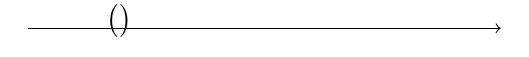
\begin{tikzpicture}
			\draw[->](-1,0)->(5,0);
			\IntervalLR{-1}{1/2}
			\def\skipInterval{0.5cm}%Khoảng cách đặt nhãn
			\IntervalGRF{}{}{\big(}{a}%Gạch xọc phải qua trái
			\IntervalLR{4}{4.8}
			\def\skipInterval{0.5cm}%Khoảng cách đặt nhãn
			\IntervalGRF{\big)}{b}{}{}%Gạch xọc phải qua trái
	\end{tikzpicture}}
	{\True 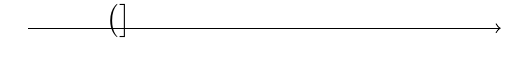
\begin{tikzpicture}
			\draw[->](-1,0)->(5,0);
			\IntervalLR{-1}{1/2}
			\def\skipInterval{0.5cm}%Khoảng cách đặt nhãn
			\IntervalGRF{}{}{\big(}{a}%Gạch xọc phải qua trái
			\IntervalLR{4}{4.8}
			\def\skipInterval{0.5cm}%Khoảng cách đặt nhãn
			\IntervalGRF{\big]}{b}{}{}%Gạch xọc phải qua trái
	\end{tikzpicture}}
	{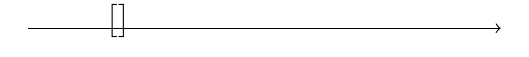
\begin{tikzpicture}
			\draw[->](-1,0)->(5,0);
			\IntervalLR{-1}{1/2}
			\def\skipInterval{0.5cm}%Khoảng cách đặt nhãn
			\IntervalGRF{}{}{\big[}{a}%Gạch xọc phải qua trái
			\IntervalLR{4}{4.8}
			\def\skipInterval{0.5cm}%Khoảng cách đặt nhãn
			\IntervalGRF{\big]}{b}{}{}%Gạch xọc phải qua trái
	\end{tikzpicture}}
	{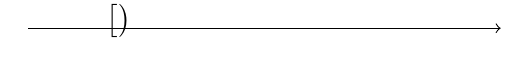
\begin{tikzpicture}
			\draw[->](-1,0)->(5,0);
			\IntervalLR{-1}{1/2}
			\def\skipInterval{0.5cm}%Khoảng cách đặt nhãn
			\IntervalGRF{}{}{\big[}{a}%Gạch xọc phải qua trái
			\IntervalLR{4}{4.8}
			\def\skipInterval{0.5cm}%Khoảng cách đặt nhãn
			\IntervalGRF{\big)}{b}{}{}%Gạch xọc phải qua trái
	\end{tikzpicture}}
	\loigiai{
	}
\end{ex}

\begin{ex}%[0D1B2]
	Tập hợp $A=\left\{x\in \mathbb{R}\big| 2>x>0 \right\}$ bằng tập hợp nào dưới đây? 
	\choice
	{$(0; 2]$}
	{\True $(0; 2)$}
	{$[0; 2]$}
	{$\left\{0; 2\right\}$}
	\loigiai{
	}
\end{ex}
\begin{ex}%[0D1B2]
	Tập hợp $A=(1;5)$ có bao nhiêu phần tử?
	\choice
	{$2$}
	{\True vô số}
	{$3$}
	{$5$}
	\loigiai{
	}
\end{ex}
\begin{ex}%[0D1K2]
	Cho tập hợp $A = [-2;1)$. Tập hợp $A$ là tập con của tập hợp nào sau đây?
	\choice{$B=[-1;2)$}
	{\True $C = \left\{x \in \mathbb{R} \mid -2 \le x < 1\right\} $}
	{$D=  \left\{x \in \mathbb{Z} \mid -2 \le x < 1\right\}$}
	{$E=  \left\{x \in \mathbb{N} \mid -2 \le x < 1\right\}$}
	\loigiai{
	}
\end{ex}

\begin{ex}%[0D1K2]
	Cho tập hợp $X = \left\{x \in \mathbb{R} \mid x > -1 \right\}.$ Tập hợp nào trong các tập hợp sau đây {\bf không} chứa tập hợp $X$?
	\choice{\True $A = [-3;7) $}
	{$ \mathbb{R}$}
	{$ B = [-3;+\infty )$}
	{$ C = [-1; +\infty)  $}
	\loigiai{
	}
\end{ex}
\begin{ex}%[0D1K2]
	Cho tập hợp $X = \left[-3;5\right]$. Biểu diễn tập hợp $X$ trên trục số ta được hình biểu diễn nào trong các hình sau  (phần không bị gạch chéo)?
	\choice{
		\True 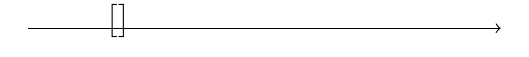
\begin{tikzpicture}
			\draw[->](-1,0)->(5,0);
			\IntervalLR{-1}{1/2}
			\def\skipInterval{0.5cm}%Khoảng cách đặt nhãn
			\IntervalGRF{}{}{\big[}{-3}%Gạch xọc phải qua trái
			\IntervalLR{4}{4.8}
			\def\skipInterval{0.5cm}%Khoảng cách đặt nhãn
			\IntervalGRF{\big]}{5}{}{}%Gạch xọc phải qua trái
	\end{tikzpicture}}
	{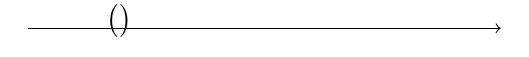
\begin{tikzpicture}
			\draw[->](-1,0)->(5,0);
			\IntervalLR{-1}{1/2}
			\def\skipInterval{0.5cm}%Khoảng cách đặt nhãn
			\IntervalGRF{}{}{\big(}{-3}%Gạch xọc phải qua trái
			\IntervalLR{4}{4.8}
			\def\skipInterval{0.5cm}%Khoảng cách đặt nhãn
			\IntervalGRF{\big)}{5}{}{}%Gạch xọc phải qua trái
	\end{tikzpicture}}
	{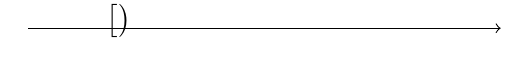
\begin{tikzpicture}
			\draw[->](-1,0)->(5,0);
			\IntervalLR{-1}{1/2}
			\def\skipInterval{0.5cm}%Khoảng cách đặt nhãn
			\IntervalGRF{}{}{\big[}{-3}%Gạch xọc phải qua trái
			\IntervalLR{4}{4.8}
			\def\skipInterval{0.5cm}%Khoảng cách đặt nhãn
			\IntervalGRF{\big)}{5}{}{}%Gạch xọc phải qua trái
	\end{tikzpicture}}
	{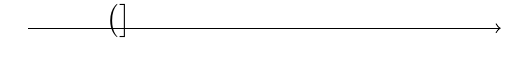
\begin{tikzpicture}
			\draw[->](-1,0)->(5,0);
			\IntervalLR{-1}{1/2}
			\def\skipInterval{0.5cm}%Khoảng cách đặt nhãn
			\IntervalGRF{}{}{\big(}{-3}%Gạch xọc phải qua trái
			\IntervalLR{4}{4.8}
			\def\skipInterval{0.5cm}%Khoảng cách đặt nhãn
			\IntervalGRF{\big]}{5}{}{}%Gạch xọc phải qua trái
	\end{tikzpicture}}
	\loigiai{
	}
\end{ex}
\begin{ex}%[0D1K2]
	Cho tập hợp $A$ được biểu diễn trên trục số như sau (phần không bị gạch chéo).
	\begin{center}
		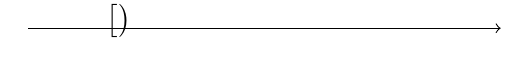
\begin{tikzpicture}
			\draw[->](-1,0)->(5,0);
			\IntervalLR{-1}{1/2}
			\def\skipInterval{0.5cm}%Khoảng cách đặt nhãn
			\IntervalGRF{}{}{\big[}{3}%Gạch xọc phải qua trái
			\IntervalLR{4}{4.8}
			\def\skipInterval{0.5cm}%Khoảng cách đặt nhãn
			\IntervalGRF{\big)}{5}{}{}%Gạch xọc phải qua trái
		\end{tikzpicture}
	\end{center}
	Khẳng định nào sau đây đúng?
	\choice{$A = \left(3;5\right)$}
	{\True $A = \left[3;5\right)$}
	{$A = \left[3;5\right]$}
	{$A = \left(3;5\right]$}
	\loigiai{
	}
\end{ex}
\begin{ex}%[0D1K2]
	Cho các tập hợp $A = \left(-1;3\right)$, $B = \left(-\infty;4\right)$ và $C = \left[-1;3\right]$. Khẳng định nào sau đây đúng?
	\choice{$B \subset A$}
	{$B \subset C$}
	{\True $C \subset B$}
	{$C \subset A$}
	\loigiai{
	}
\end{ex}

\begin{ex}%[0D1K2]
	Cho các số thực $a, b, c, d$ thoả mãn $a<b<c<d$. Hãy chọn mệnh đề \textbf{sai} trong các mệnh đề sau:
	\choice
	{\True $(a;c)\subset (c;d)$}
	{$(b;c)\subset (b;d)$}
	{$(b;c)\subset (a;d)$}
	{$(a;c)\subset (a;d)$}
	\loigiai{
	}
\end{ex}

\begin{ex}%[0D1K3]
	Cho các số thực $a$, $b$, $c$, $d$ và $a<b<c<d$. Trong các mệnh đề sau, mệnh đề nào đúng?
	\choice
	{\True$\left(a;c\right)\cap\left(b;d\right)=\left(b;c\right)$}
	{$\left(a;c\right)\cap\left[b;d\right)=\left[b;c\right]$}
	{$\left(a;c\right)\cap\left[b;d\right)=\left[b;c\right]$}
	{$\left(a;c\right)\cup\left(b;d\right)=\left(b;c\right)$}
	\loigiai{
	}
\end{ex}

\begin{ex}%[0D1B3]
	Trên trục số, phần không bị gạch biểu diễn tập hợp nào trong các tập hợp sau?
	\begin{center}
		\begin{tikzpicture}[xscale=0.5,thick,>=stealth']
			\draw[->](-5,0)->(6,0);
			\IntervalRF{]}{-2}{(}{2}
		\end{tikzpicture}
	\end{center}
	\choice
	{$\left( {-\infty; -2}\right]\cup \left[ {2;+\infty}\right)$}
	{\True $\left( {-\infty; -2}\right]\cup \left( {2;+\infty}\right)$}
	{$\left( {-\infty; -2}\right)\cup \left[ {2;+\infty}\right)$}
	{$\left( {-\infty; -2}\right)\cup \left( {2;+\infty}\right)$}
	\loigiai{
	}
\end{ex}
\begin{ex}%[0D1B3]
	Cho hai tập hợp $X=\left[ -2;3 \right]$ và  $Y=\left( 1;5 \right]$. Tìm tập hợp $X\backslash Y$.
	\choice
	{\True $\left[ -2;1 \right]$}
	{$\left( 3;5 \right]$}
	{$\left[ -2;1 \right)$}
	{$\left( -2;1 \right]$}
	\loigiai{
	}
\end{ex}

\begin{ex}%[0D1K3]
	Cho hai tập hợp $A=\left\{ x\in \mathbb{R}\big|x+2\geq 0 \right\}$ và $B=\left\{ x\in \mathbb{R}\big|5-x\geq 0 \right\}$. Tìm tập hợp $A\cap B$. 
	\choice
	{\True $\left[ -2;5 \right]$}
	{$\left[ -2;6 \right]$}
	{$\left[ -5;2 \right]$}
	{$\left( -2;+\infty  \right)$}
	\loigiai{
		Ta có
		\begin{itemize}
			\item [$\bullet$] $x+2 \ge 0 \Leftrightarrow x \ge -2$ và $x \in \mathbb{R}$ nên $A=[-2;+\infty)$.
			\item [$\bullet$] $5-x \ge 0 \Leftrightarrow x \le 5$ và $x \in \mathbb{R}$ nên $B=(-\infty;5]$.
		\end{itemize} 
		Suy ra $A\cap B = \left[ -2;5 \right].$
	}
\end{ex}

\begin{ex}%[0D1K3]
	Cho hai tâp hợp $A = \left[-5; 3\right); B = \left[0; 2\right)$. Tìm tập hợp $\mathbb{R} \setminus \left( B \cap A\right)$.
	\choice
	{\True $\left(-\infty; 0\right) \cup \left[2; +\infty\right)$}
	{$\left[0; 2\right)$}
	{$\left[2; +\infty\right)$}
	{$\left(-\infty; 0\right)$}
	\loigiai{Do $A \cap B = \left[0; 2\right)$ nên $\mathbb{R} \setminus (A \cap B) = (-\infty; 0) \cup [2; +\infty)$}
\end{ex}

\begin{ex}%[0D1B3]
	Cho tập hợp $A=\left( 2;+\infty  \right)$. Tìm tập hợp $C_{\mathbb{R}} {A}$.  
	\choice
	{$\left[ 2;+\infty  \right)$}
	{$\left( 2;+\infty  \right)$}
	{\True $\left( -\infty ;2 \right]$}
	{$\left( -\infty ;-2 \right]$}
	\loigiai{
	}
\end{ex}

\begin{ex}%[0D1B3]
	Cho các tập hợp sau $A =\left(-1; 5\right], B = \left(2; 7\right)$. Tìm tập hợp $A \setminus B$.
	\choice
	{\True $\left(-1; 2\right]$}
	{$\left(2; 5\right]$}
	{$\left(-1; 7\right)$}
	{$\left(-1; 2\right)$}
	\loigiai{
	}
\end{ex}

\begin{ex}%[0D1K3]
	Cho hai tập hợp $A=\left\{ x\in \mathbb{R}\big| x+2\geq 0 \right\}$ và $B=\left\{ x\in \mathbb{R}\big| 5-x\geq 0 \right\}$. Tìm tập hợp $A \setminus B$. 
	\choice
	{$\left[ -2;5 \right]$}
	{$\left[ -2;6 \right]$}
	{\True $\left( 5;+\infty  \right)$}
	{$\left( 2;+\infty  \right)$}
	\loigiai{
		Ta có
		\begin{itemize}
			\item [$\bullet$] $x+2 \ge 0 \Leftrightarrow x \ge -2$ và $x \in \mathbb{R}$ nên $A=[-2;+\infty)$.
			\item [$\bullet$] $5-x \ge 0 \Leftrightarrow x \le 5$ và $x \in \mathbb{R}$ nên $B=(-\infty;5]$.
		\end{itemize} 
		Suy ra $A \setminus B= \left( 5;+\infty  \right)$.
	}
\end{ex}

\begin{ex}%[0D1K3]
	Biểu diễn trên trục số của tập hợp  $ \left[ -3;1\right) \cap \left( {-2;4}\right]$ là hình nào?
	\def\dotEX{}
	\choice
	{\True \begin{tikzpicture}[xscale=0.5,thick,>=stealth']
			\draw[->](-5,0)->(6,0);
			\IntervalLR{-5}{-2}
			\IntervalGRF{}{}{(}{-2}
			\IntervalLR{1}{6}
			\IntervalGRF{)}{1}{}{}
	\end{tikzpicture}}
	{\begin{tikzpicture}[xscale=0.5,thick,>=stealth']
			\draw[->](-5,0)->(6,0);
			\IntervalLR{-5}{-3}
			\IntervalGRF{}{}{[}{-3}
			\IntervalLR{4}{6}
			\IntervalGRF{]}{4}{}{}
	\end{tikzpicture} }
	{\begin{tikzpicture}[xscale=0.5,thick,>=stealth']
			\draw[->](-5,0)->(6,0);
			\IntervalLR{-5}{-3}
			\IntervalGRF{}{}{[}{-3}
			\IntervalLR{1}{6}
			\IntervalGRF{)}{1}{}{}
	\end{tikzpicture}}
	{\begin{tikzpicture}[xscale=0.5,thick,>=stealth']
			\draw[->](-5,0)->(6,0);
			\IntervalLR{-5}{-2}
			\IntervalGRF{}{}{(}{-2}
			\IntervalLR{4}{6}
			\IntervalGRF{]}{4}{}{}
	\end{tikzpicture}}
	\loigiai{
		Ta có $ \left[ -3;1\right) \cap \left( {-2;4}\right]=(-2;1).$
	}
\end{ex}

\begin{ex}%[0D1K3]
	Biểu diễn trên trục số của tập hợp $ \left( 0;2\right) \cup \left[ {-1;1}\right)$ là hình nào?
	\def\dotEX{}
	\choice
	{\begin{tikzpicture}[xscale=0.5,thick,>=stealth']
			\draw[->](-5,0)->(6,0);
			\IntervalLR{-5}{-1}
			\IntervalGRF{}{}{(}{-1}
			\IntervalLR{2}{6}
			\IntervalGRF{]}{2}{}{}
	\end{tikzpicture}}
	{\begin{tikzpicture}[xscale=0.5,thick,>=stealth']
			\draw[->](-5,0)->(6,0);
			\IntervalLR{-5}{-1}
			\IntervalGRF{}{}{[}{-1}
			\IntervalLR{2}{6}
			\IntervalGRF{]}{2}{}{}
	\end{tikzpicture} }
	{\begin{tikzpicture}[xscale=0.5,thick,>=stealth']
			\draw[->](-5,0)->(6,0);
			\IntervalLR{-5}{-1}
			\IntervalGRF{}{}{(}{-1}
			\IntervalLR{2}{6}
			\IntervalGRF{)}{2}{}{}
	\end{tikzpicture}}
	{\True \begin{tikzpicture}[xscale=0.5,thick,>=stealth']
			\draw[->](-5,0)->(6,0);
			\IntervalLR{-5}{-1}
			\IntervalGRF{}{}{[}{-1}
			\IntervalLR{2}{6}
			\IntervalGRF{)}{2}{}{}
	\end{tikzpicture}}
	\loigiai{
		Ta có $ \left( 0;2\right) \cup \left[ {-1;1}\right)=[-1;2).$
	}
\end{ex}

\begin{ex}
	Cho hai tập hợp $A=[-1 ; 4], B=[m+1 ; m+3]$ với $m$ là tham số. Tìm tất cả các giá trị của $m$ để $B \backslash A=\varnothing$.
	\choice
	{$m<0$ hoặc $m>3$}
	{$m<-5$ hoặc $m>3$}
	{\True $m<-4$ hoặc $m>3$}
	{$m<-2$ hoặc $m>5$}
	\loigiai{
		$B \backslash A=\varnothing \Leftrightarrow \hoac{&m+3<-1\\&m+1>4} \Leftrightarrow \hoac{&m<-4\\&m>3}$
	}
\end{ex}

\begin{ex}%[0D1K2]
	Tìm tất cả các giá trị nguyên của tham số $m$ để tập hợp $\left(1;m\right)$ chứa đúng 1 số nguyên dương.
	\choice
	{$m=2$}
	{$m>2$}
	{\True$m=3$}
	{$m=4$}
	\loigiai{
		Các số nguyên dương lớn hơn 1 sẽ là 2; 3; 4,... Suy ra, để $\left(1;m\right)$  chỉ chứa 1 số nguyên dương thì giá trị nguyên cần tìm của $m$ là $m=3$.
	}
\end{ex}
\begin{ex}%[0D1K2]
	Tìm tất cả các giá trị nguyên của tham số  $m$ để tập hợp $\left(1;m\right)$ chứa đúng 2 số nguyên dương.
	\choice
	{$m=2$}
	{$m>2$}
	{$m=3$}
	{\True $m=4$}
	\loigiai{
		Các số nguyên dương lớn hơn 1 sẽ là 2; 3; 4,... Suy ra, để $\left(1;m\right)$  chỉ chứa 1 số nguyên dương thì giá trị nguyên cần tìm của $m$ là $m=4$.
	}
\end{ex}

\begin{ex}%[0D1K4]
	Cho hai tập hợp $A = \left[ {1;3} \right]$ và $B = \left[ {m;m + 1} \right]$. Tìm tất cả các giá trị của tham số $ m $ để $B \subset A$.
	\choice
	{$ m=1 $}
	{$ m=2 $}
	{$ 1<m<2 $}
	{\True $ 1 \leqslant m \leqslant 2 $}
	\loigiai{ Ta có $B\subset A$ khi và chỉ khi $\heva{& m \geq 1 \\ & m+1 \leq 3} \Leftrightarrow 1 \leq m \leq 2$.
		
	}
\end{ex}

\begin{ex}%[0D1G3]
	Cho hai tập hợp $A = \left[ m; m + 2\right]; B =\left[ -1; 2\right]$. Tìm tất cả các giá trị thực của tham số $m$ để $A \subset B$.
	\choice
	{$\hoac{& m \leq -1 \\ & m \geq 0}$}
	{\True $-1 \leq m \leq 0$}
	{$1 \leq m \leq 2$}
	{$\hoac{& m < -1\\& m > 2}$}
	\loigiai{Để $A \subset B$ thì $\heva{& m \geq -1\\& m + 2 \leq 2} \Leftrightarrow \heva{& m \geq -1 \\ & m \leq 0}$.}
\end{ex}

\begin{ex}%[0D1G3]
	Cho hai tập hợp $A =\left( -\infty; m -1\right], B =\left[ 1; +\infty \right)$. Tìm tất cả các giá trị thực của tham số $m$ để $A \cap B = \varnothing$.
	\choice
	{$m > -1 $}
	{$m \geq -1$}
	{$m \leq 2$}
	{\True $m < 2$}
	\loigiai{Để $A \cap B = \varnothing$ thì $m - 1 < 1 \Rightarrow m < 2$.}
\end{ex}

\begin{ex}%[0D1G3]
	Cho các tập $B = \left\{x \in \mathbb{R} \,|\,-5 \leq x \leq 5\right\}$;$C = \left\{x \in \mathbb{R} \,|\, x \leq a\right\}, \,\, \text{và}\,\, D = \left\{x \in \mathbb{R} \,|\, x \geq b\right\}$. Xác định $a, b$ biết $C \cap B$ và $D \cap B$ là các đoạn có độ dài lần lượt bằng $5$ và $9$.
	\choice
	{\True $a = 0; b = -4$}{$a = 5; b = 9$}{$a = -4; b = 0$}{$a = -5; b = 5$}
	\loigiai{Ta có $B = \left[-5; 5\right]; C = \left(-\infty; a\right]; D = \left[b; +\infty\right)$.\\
		Theo giả thiết thì $C \cap B$ và $D \cap B$ khác $\varnothing$ nên $C \cap B = \left[-5; a\right]$ và $D \cap B = \left[b; 5\right]$\\
		Theo yêu cầu đề bài: $\heva {& a + 5 = 5\\& 5 - b = 9} \Leftrightarrow \heva {& a = 0\\ & b = -4}$.}
\end{ex}
% \centerline{\textbf{---HẾT---}}
\Closesolutionfile{ans}